\documentclass[a4paper,12pt]{article}
\usepackage{graphicx} 
\usepackage{amsmath} 
\usepackage{amssymb} 
\usepackage{geometry} 
\usepackage{fancyhdr} % for headers and footers
\usepackage{caption} % for customizing captions
\usepackage{subcaption}
\usepackage{setspace} 
\usepackage[bottom]{footmisc}
\usepackage{adjustbox}
\usepackage{placeins}
\usepackage{float}
\usepackage[nopatch=item]{microtype}
\usepackage{enumitem} % for customizing lists
\usepackage[backend=biber]{biblatex} % for bibliography
\usepackage[colorlinks,linkcolor=blue,citecolor=blue,urlcolor=blue]{hyperref}
\addbibresource{Sci. Data_01.bib} % specify your bibliography file

\setlength{\parindent}{1.27cm} % Indent first line of each paragraph by 1.27 cm (0.5 inches)

\geometry{margin=1in}
\setlength{\parindent}{0pt}
\setlength{\parskip}{6pt}
\doublespacing

 
\pagestyle{fancy}
\fancyhf{}
\fancyhead[L]{\leftmark}
\fancyfoot[C]{\thepage}

\begin{document}


\section{Results}
\subsection{Part 1}
\subsubsection{Original signal and its Fourier transform}
\par Once collected the data, we procede with the visualization of the data 
in graphical form. The following Fig (\ref{plot:raw_signal_and_noise}) 
shows the signal saved from the oscilloscope without any data processing. 
We can compare this plot with the image acquired directly from the oscilloscope
in Fig (\ref{fig:sin+noise_signal}) and check for their similarity.
\begin{figure}[H]
    \centering
    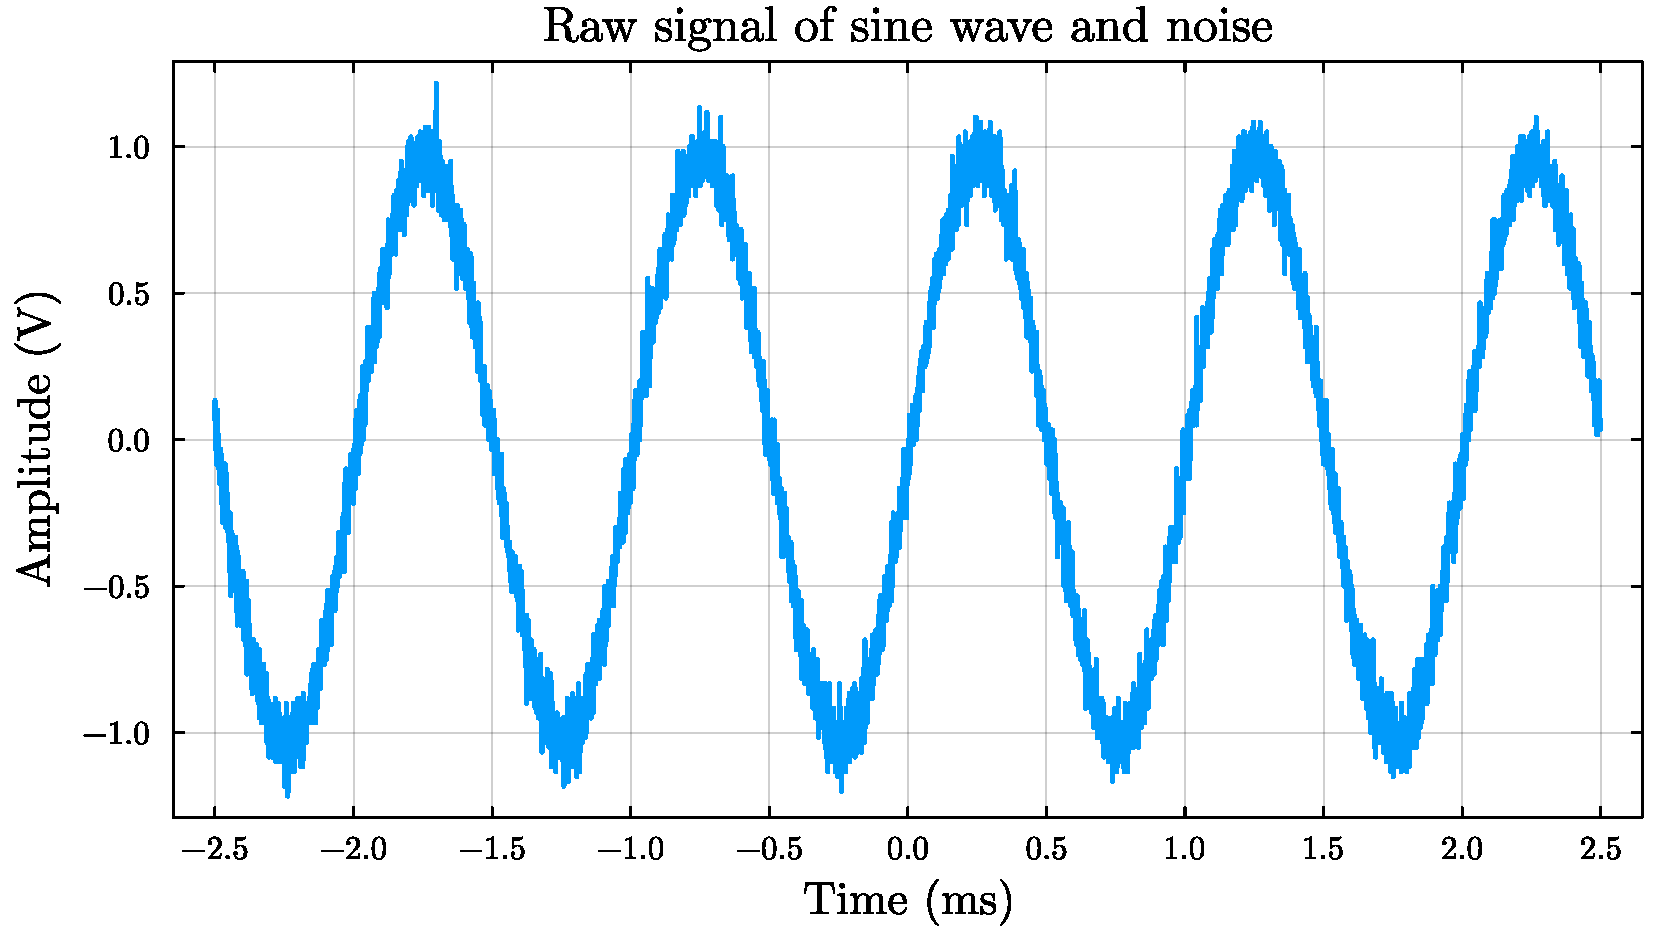
\includegraphics[width=1\textwidth]{signal01.pdf}
    \caption{One of our saved signal, composed of one sine wave and some noise.}
    \label{plot:raw_signal_and_noise}
\end{figure}

\par As our second step, we compute the Fourier transform of the previous signal, 
without using any windowing function. To do so, we take advantage of the library
"FFTW" of the julia programming language, this library implements both the
complex and real fourier transform, among with the inverse fourier transform 
and many other methods. For this experiment we will use the complex fourier transform.

\par After the transformation, we obtain an array of complex values. We will consider the
modulus of these numbers (which is the amplitude of the given frequency). Furthermore, 
we must say that the transform has non-zero values both in the positive and in the 
negative frequency axis. Our signal is of course made from real world data 
(in other words, real numbers), hence we can say that the final transformation will 
be an even function and the data on the negative side of the frequency axis will be 
a reflection of the data on the positive side of the same axis.

\par If we plot the values on the positive side only, we obtain the graph shown in 
Fig (\ref{plot:Fourier_signal}).
\begin{figure}[H]
    \centering
    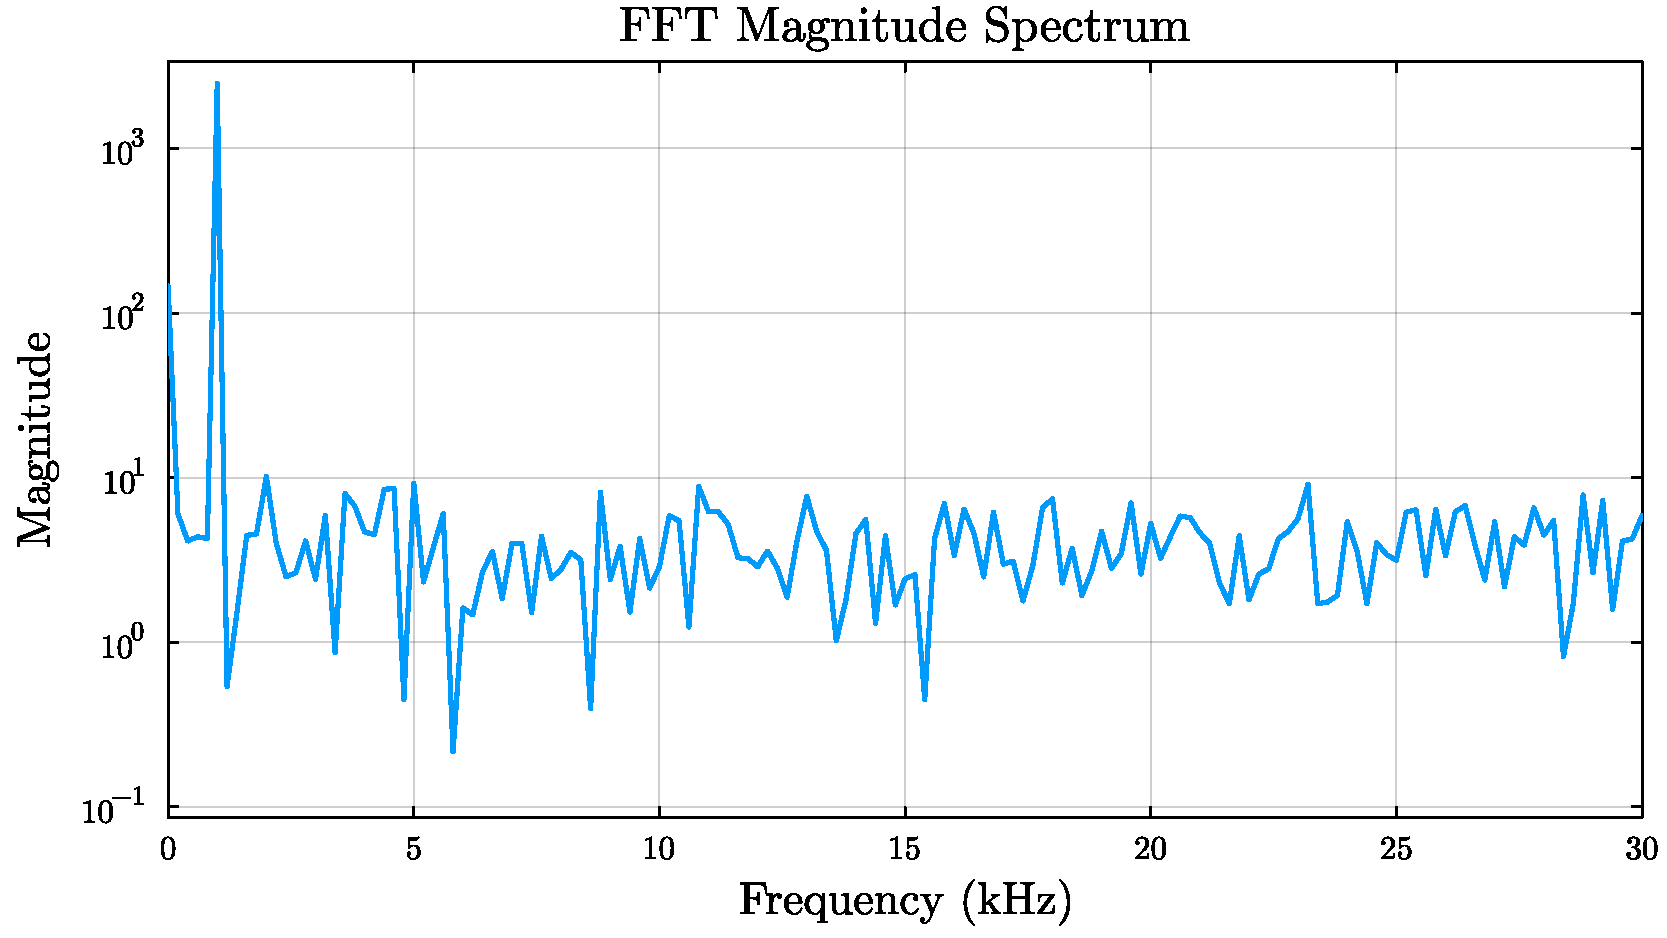
\includegraphics[width=1\textwidth]{fft01.pdf}
    \caption{Fast Fourier Transform of the signal}
    \label{plot:Fourier_signal}
\end{figure}
\begin{figure}[H]
    \centering
    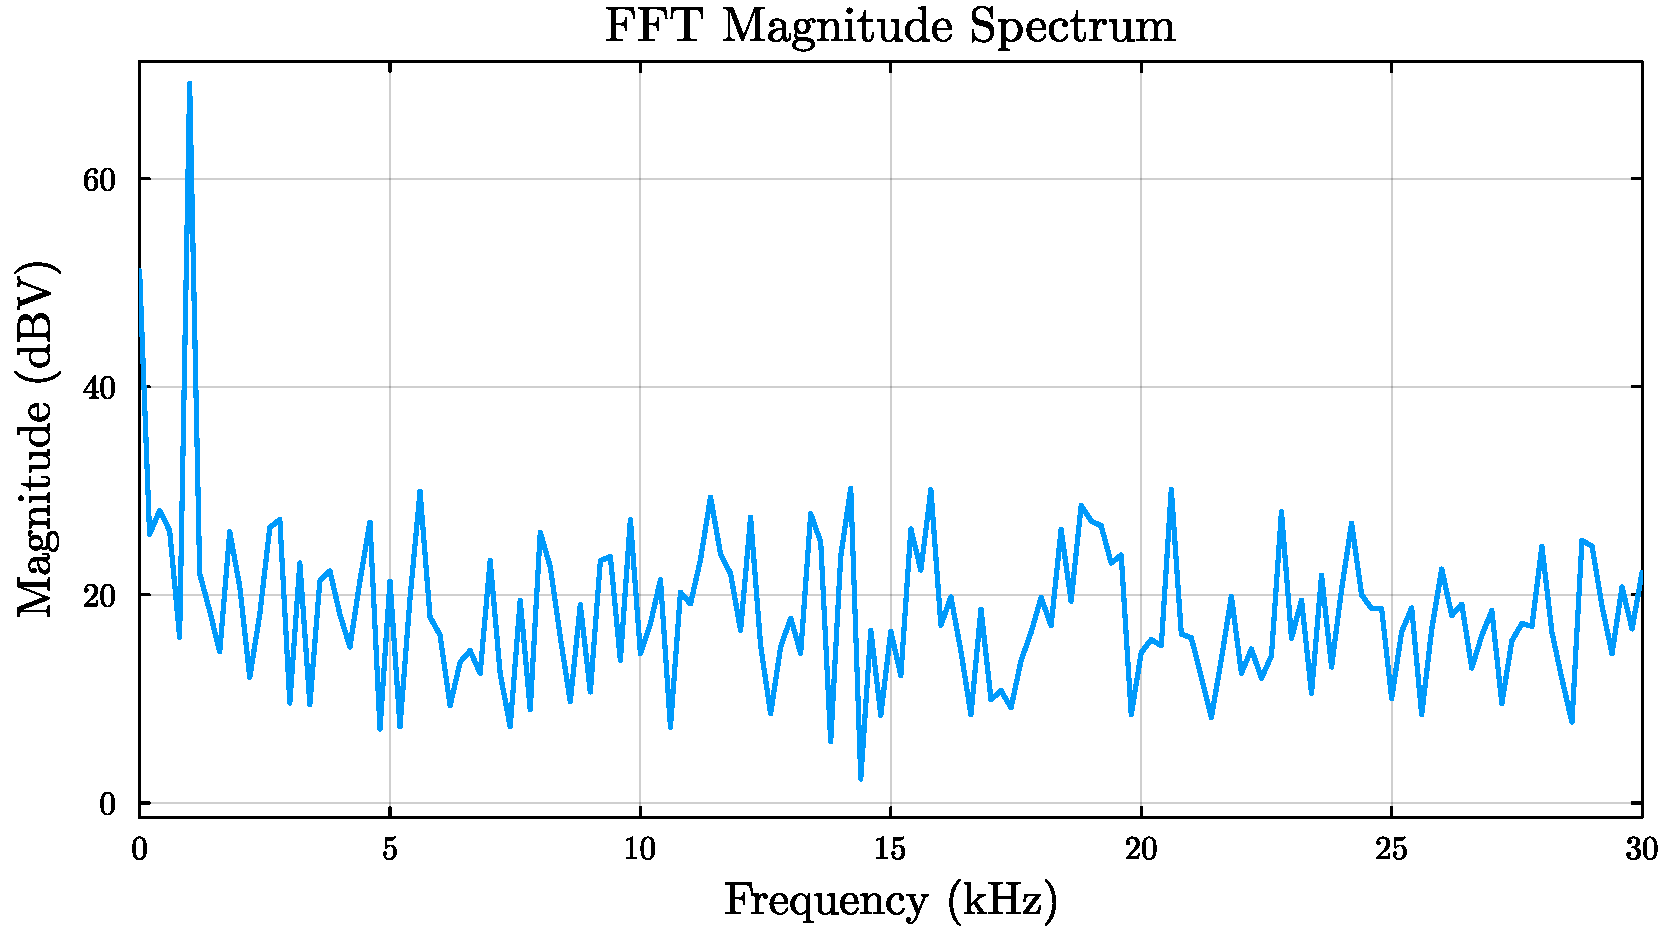
\includegraphics[width=1\textwidth]{fft01_dBV.pdf}
    \caption{Fast Fourier Transform of the signal in dBV}
    \label{plot:Fourier_signal_dBV}
\end{figure}

\par The plot in Fig (\ref{plot:Fourier_signal_dBV}) shows the Fourier transform in dBV.


\subsubsection{Peak cutoff and inverse Fourier transform }
\par We can now proceed in the selection of the frequencies which correspond to 
the noise. This step is equivalent to a peak removal, since we know that the signal 
which we are studying is a single sine wave. In practice, we modify the value of 
the Fourier transform in the position of the peak. We set this value to the mean 
of the transform in a big enought range (we use the interval $I$ from $1166$ to $4500$ Hz). 
We must remember to keep the transformation an even function, so we also modify the 
value of the transform for the negative frequency to the same value. In formulas, 
we impose 
\[
\begin{cases}
    \mathcal{F}(1000\, Hz) = \left\langle \mathcal{F}(f) \right\rangle_I \\
    \mathcal{F}(-1000\, Hz) = \mathcal{F}(1000\, Hz)
\end{cases}.
\]

\par We can now evaluate the inverse transform in order to reconstruct the original noise.
We have a plot for the reconstructed noise in Fig (\ref{plot:Only_noise}).
\begin{figure}[H]
    \centering
    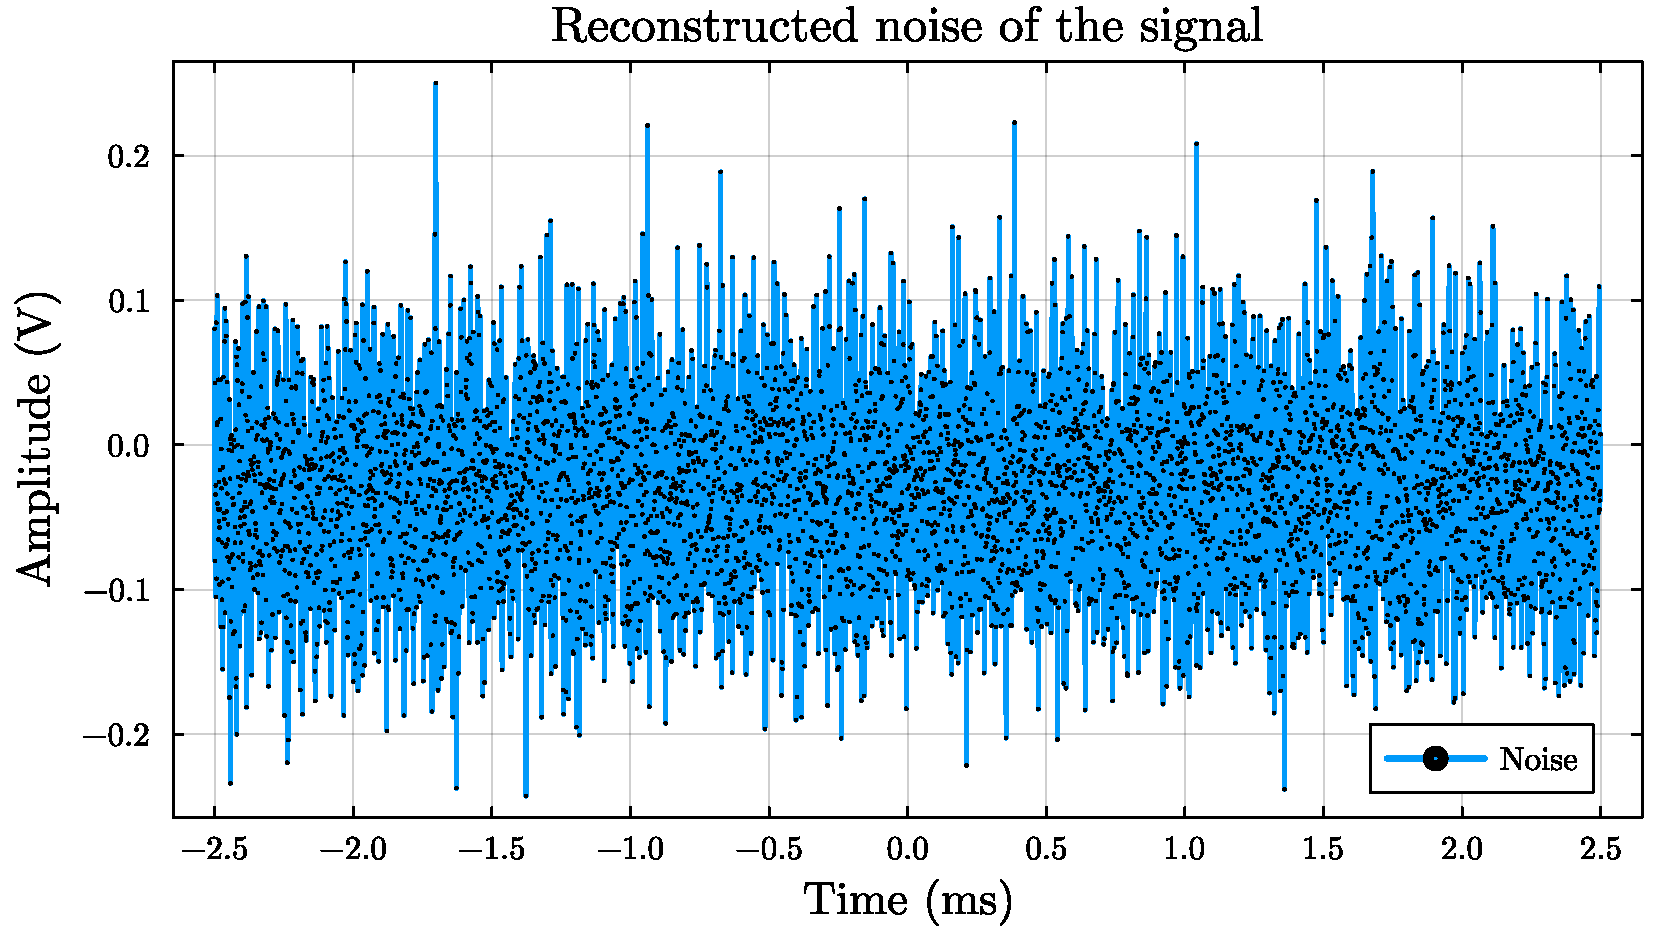
\includegraphics[width=1\textwidth]{signal01_only_noise.pdf}
    \caption{Reconstructed noise obtained from the inverse Fourier transform}
    \label{plot:Only_noise}
\end{figure}

\subsubsection{Statistical analysis of the reconstructed noise}
\par From the data obtained from the previos section, we can conduct 
a brief statistical analysis. The main purpose of this section is to 
check whether the noise obtained can be classified as white noise, that is 
noise that follows a normal distribution (also called Gaussian distribution).

\par We begin by calculating the mean ($\mu$) and the standard deviation 
($\sigma$) of the data, obtaining $\mu = -0.02925 \, mV$ and $\sigma = 0.06231 mV$.
As expected, the noise has a mean value very close to zero and the error is 
bigger than the mean, which means that the zero is inside the confidence 
range of $68\%$.  

\par We will now use the chi squared test to check how well the normal 
distribution fits our data. The Fig (\ref{plot:Hist_Gauss}) lets us see the expected 
values for this distribution in overlay with the normalized histogram 
of the data from the noise.
\begin{figure}[H]
    \centering
    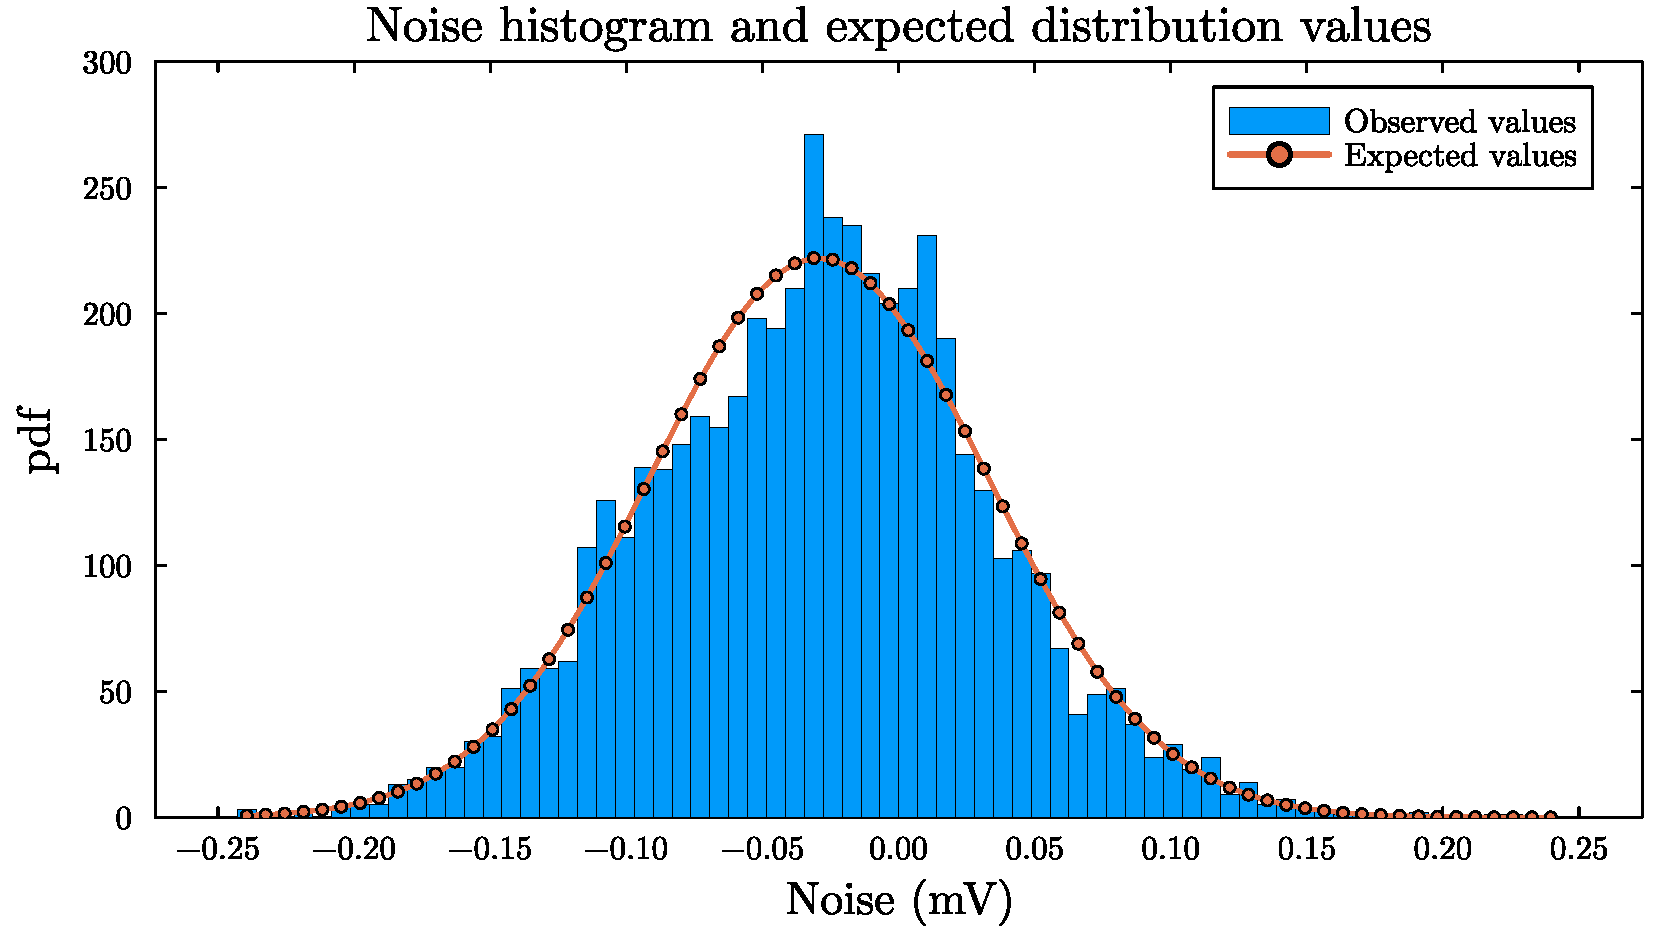
\includegraphics[width=1\textwidth]{Noise_hist_and_Normal_distr_expected_v.pdf}
    \caption{Histogram of the noise in overlay with the expected values given by the Gaussian distribution.}
    \label{plot:Hist_Gauss}
\end{figure}

\par Evaluating the chi squared gives us a result of $\chi^2 = 149.77$, 
with $d=70-3=67$ degrees of freedom. We can now obtain the reduced 
chi squared $\tilde{\chi}^2 = \chi^2 / d = 2.2354$. In this case, 
the probability to obtain a  $\chi^2$ ... is less than $0.05\%$, 
hence the distridution does not represent at all the collected data.
The Table (\ref{tab:summary_table}) 
sums up all the statistical data collected in this section.

\begin{table}[h]
    \centering
    \begin{tabular}{|c|c|}
        \hline
        Quantity & Value \\
        \hline
        Mean ($\mu$) & $-0.02925 \, mV$ \\
        \hline
        Standard error ($\sigma$) & $0.06231 mV$ \\
        \hline
        Degrees of freedom ($d$) & $67$ \\
        \hline
        Chi squared ($\chi^2$) & $149.77$ \\
        \hline
        Reduced chi squared ($\tilde{\chi}^2$) & $2.2354$ \\
        \hline
    \end{tabular}
    \caption{Summary table for the statistical quantities}
    \label{tab:summary_table}
\end{table}


\subsection{Part 2}
\subsubsection{Evaluation of the mean of multiple signals}
\par After the first part on the statistical analysis of the noise of a single signal, 
we proceed with the study of the treatment of the noise using multiple signals. 
In particular, we will make use of all 32 different datasets of the same signal to 
verify whether the error on the signal will fall off as the square root of the number of measures.

\par We begin from a graph, Fig (\ref{plot:Noise_decay_only_noise}), where we show the 
reconstructed noise obtained averaging different numbers of datasets. It's important to say 
that we first reconstruct the noise for every dataset, then we apply the average over these results. 
Here the decay of the noise is very clear to see. 
A similar plot for the signal is presented in Fig (\ref{plot:Noise_decay_signal}) in Appendix A.
\begin{figure}[H]
    \centering
    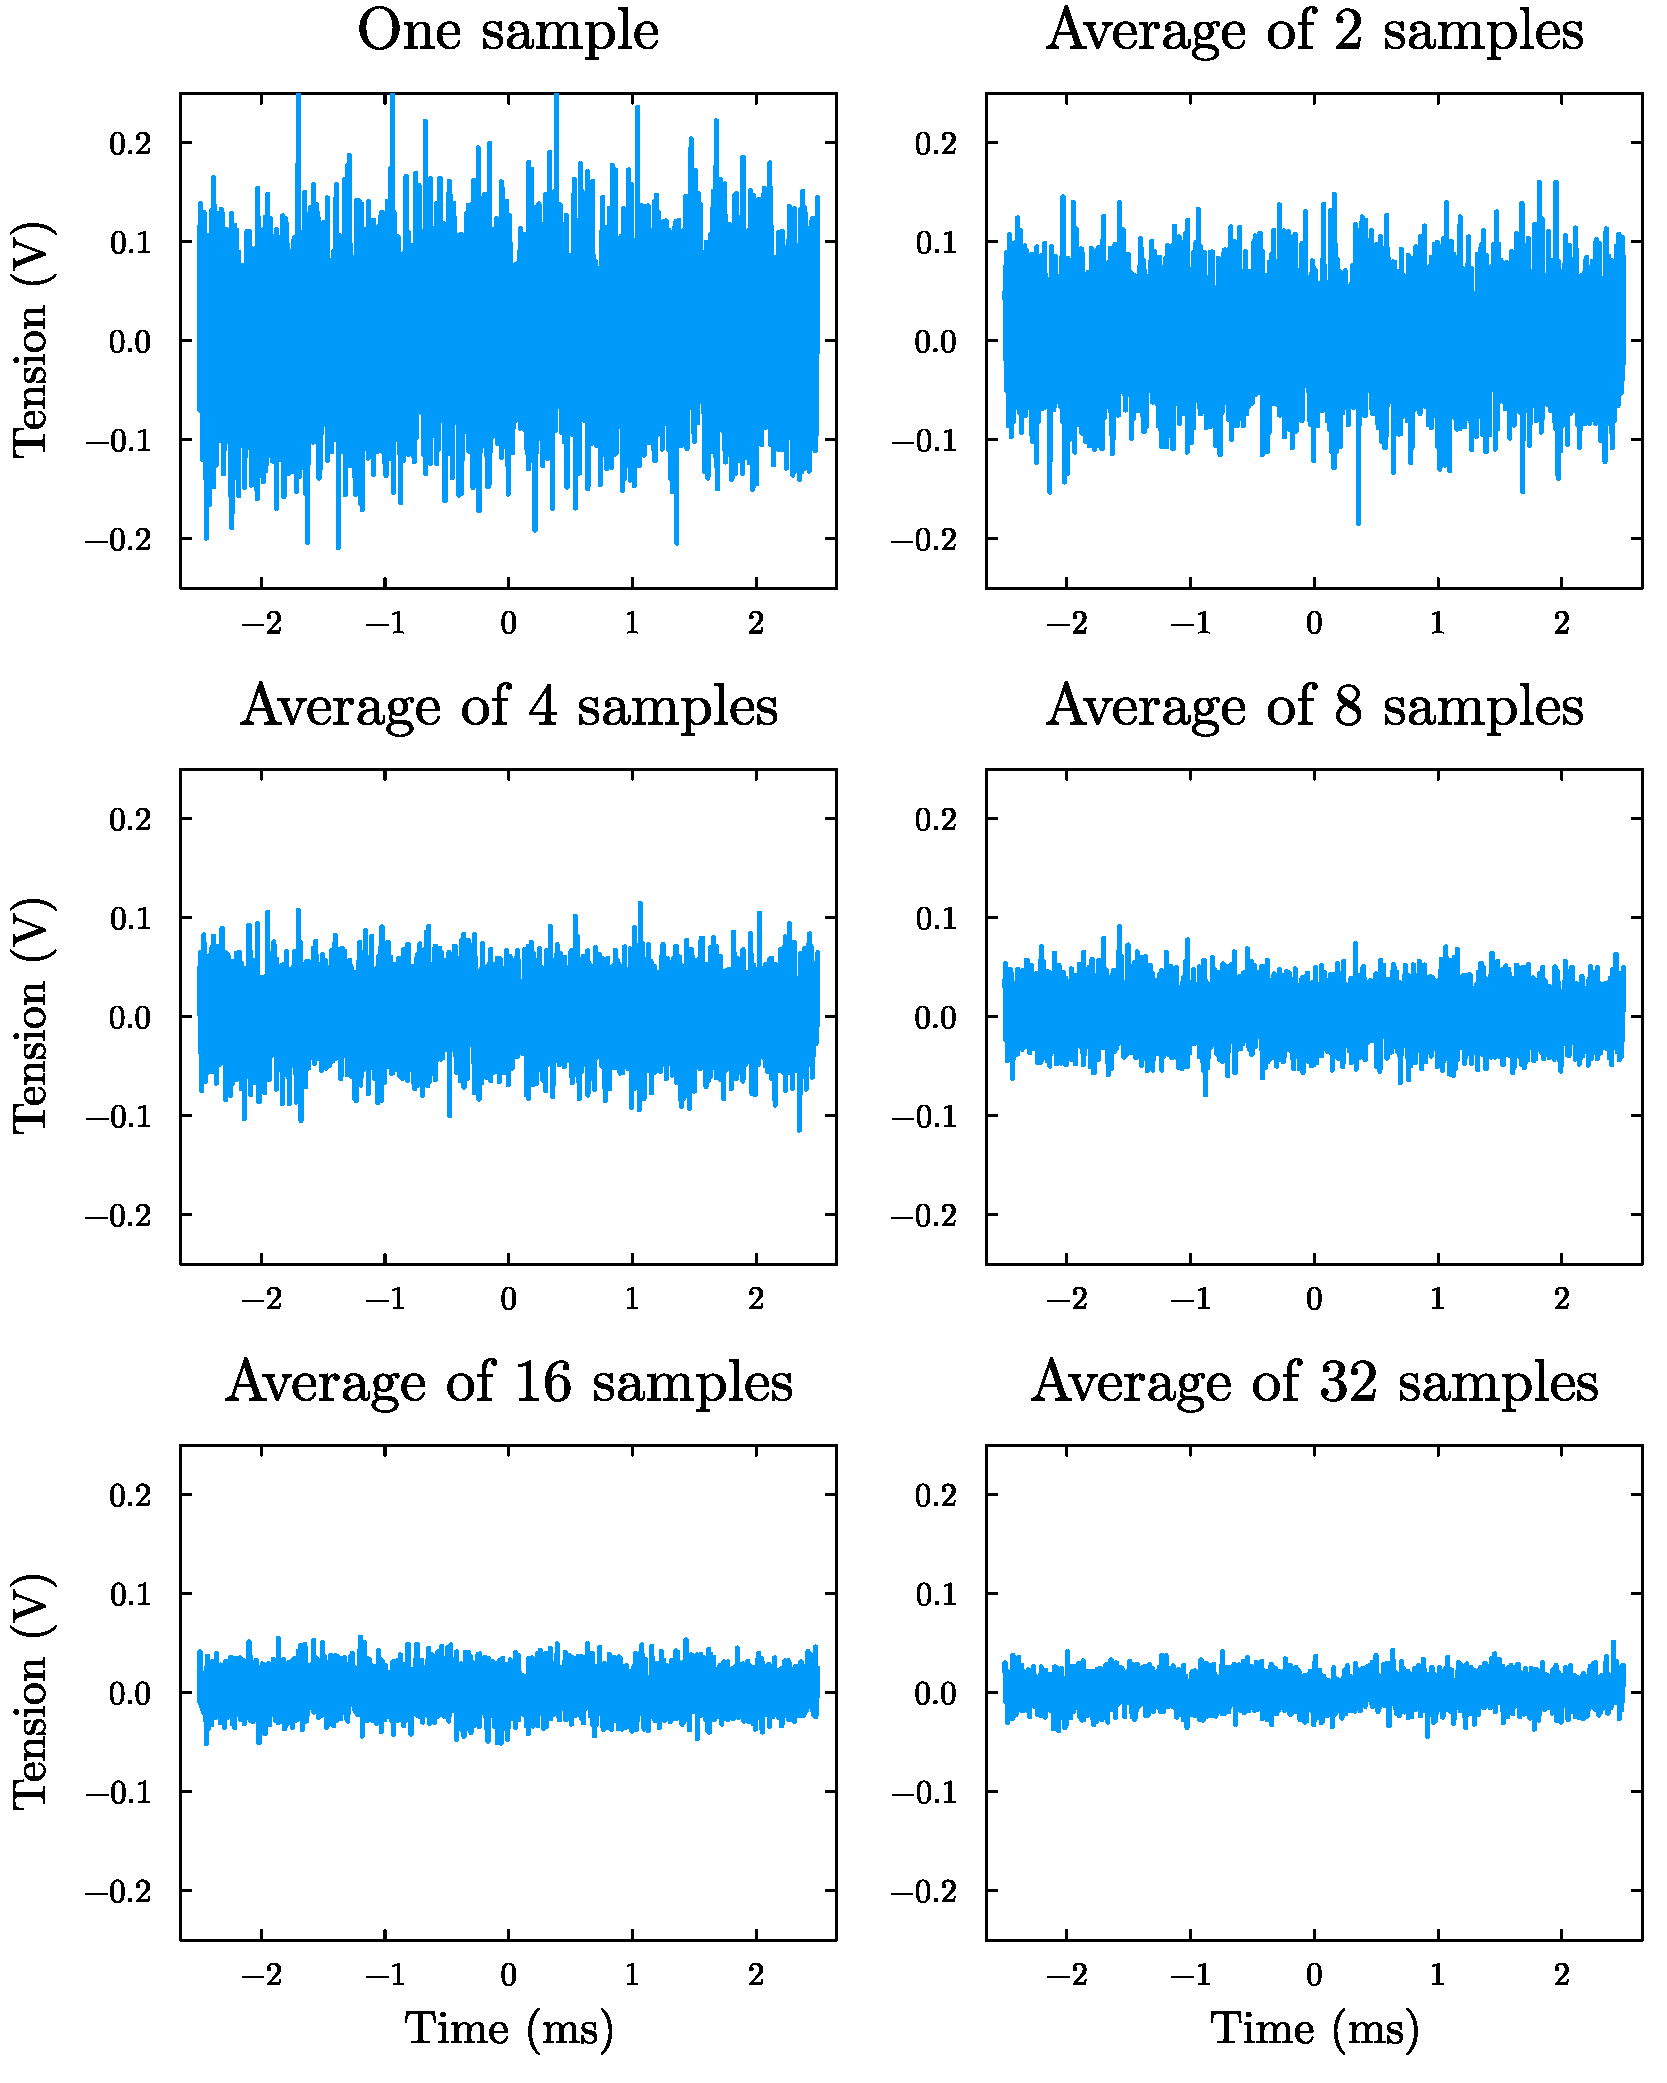
\includegraphics[width=1\textwidth]{Error_fix.pdf}
    \caption{Reconstructed noise obtained from the average of different numbers of noise datasets.}
    \label{plot:Noise_decay_only_noise}
\end{figure}

\par We then conduct some statistical analysis over the data in 
Fig (\ref{plot:Noise_decay_only_noise}), that is the evaluation of the standard error.
The results are presented in the Table (\ref{tab:sigma_error}).

\begin{table}[h]
    \centering
    \begin{tabular}{|c|c|}
        \hline
        Average of \# datasets & Standard error \\
        \hline
        1 & $0.06237$ \\
        2 & $0.04435$ \\
        4 & $0.03121$ \\
        8 & $0.02233$ \\
        16 & $0.01598$ \\
        32 & $0.01180$ \\
        \hline
    \end{tabular}
    \caption{Variation of the standard error of the reconstructed noise in function of the number of datasets condidered for the mean.}
    \label{tab:sigma_error}
\end{table}

\par We will use this data to verify our assumption, so we will assume a power law
that fits all these points. We will use the least square method applied to the 
power law case in order to find the exponent, which we expect to be approximately $- \frac{1}{2}$.
The Fig (\ref{plot:error_fit}) lets us have a look at our fit.
\begin{figure}[H]
    \centering
    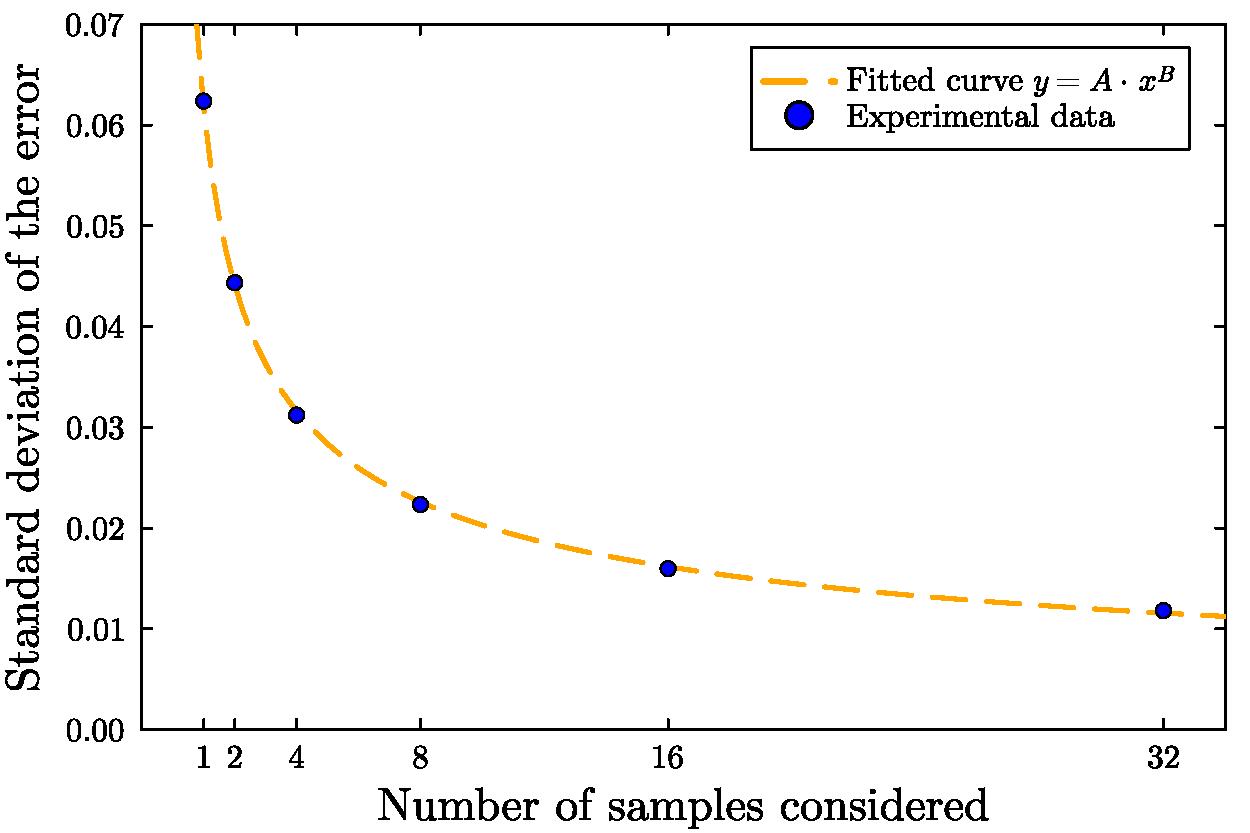
\includegraphics[width=0.7\textwidth]{Std_error.pdf}
    \caption{The standard errors of the noise and the best power law fit.}
    \label{plot:error_fit}
\end{figure}

\par The parameters for this fit and their error are reported in Table (\ref{tab:powerlaw_results}).

\begin{table}[h]
    \centering
    \begin{tabular}{|c|c|c|}
        \hline
        Parameter & Value & Error (if necessary) \\
        \hline
        $A$ & $-2.785$ & $0.011$ \\
        $B$ & $-0.4831$ & $0.0054$ \\
        $R^2$ & $0.9995$ & $/$ \\
        \hline
    \end{tabular}
    \caption{All the parameter for the power law fit $y=A \cdot x^B$.}
    \label{tab:powerlaw_results}
\end{table}

We can see how the vaue for the parameter $B$, which is the exponent, 
is very close to the expected value of $-0.5$. 






\newpage
\section{Appendix A: More figures}
\begin{figure}[H]
    \centering
    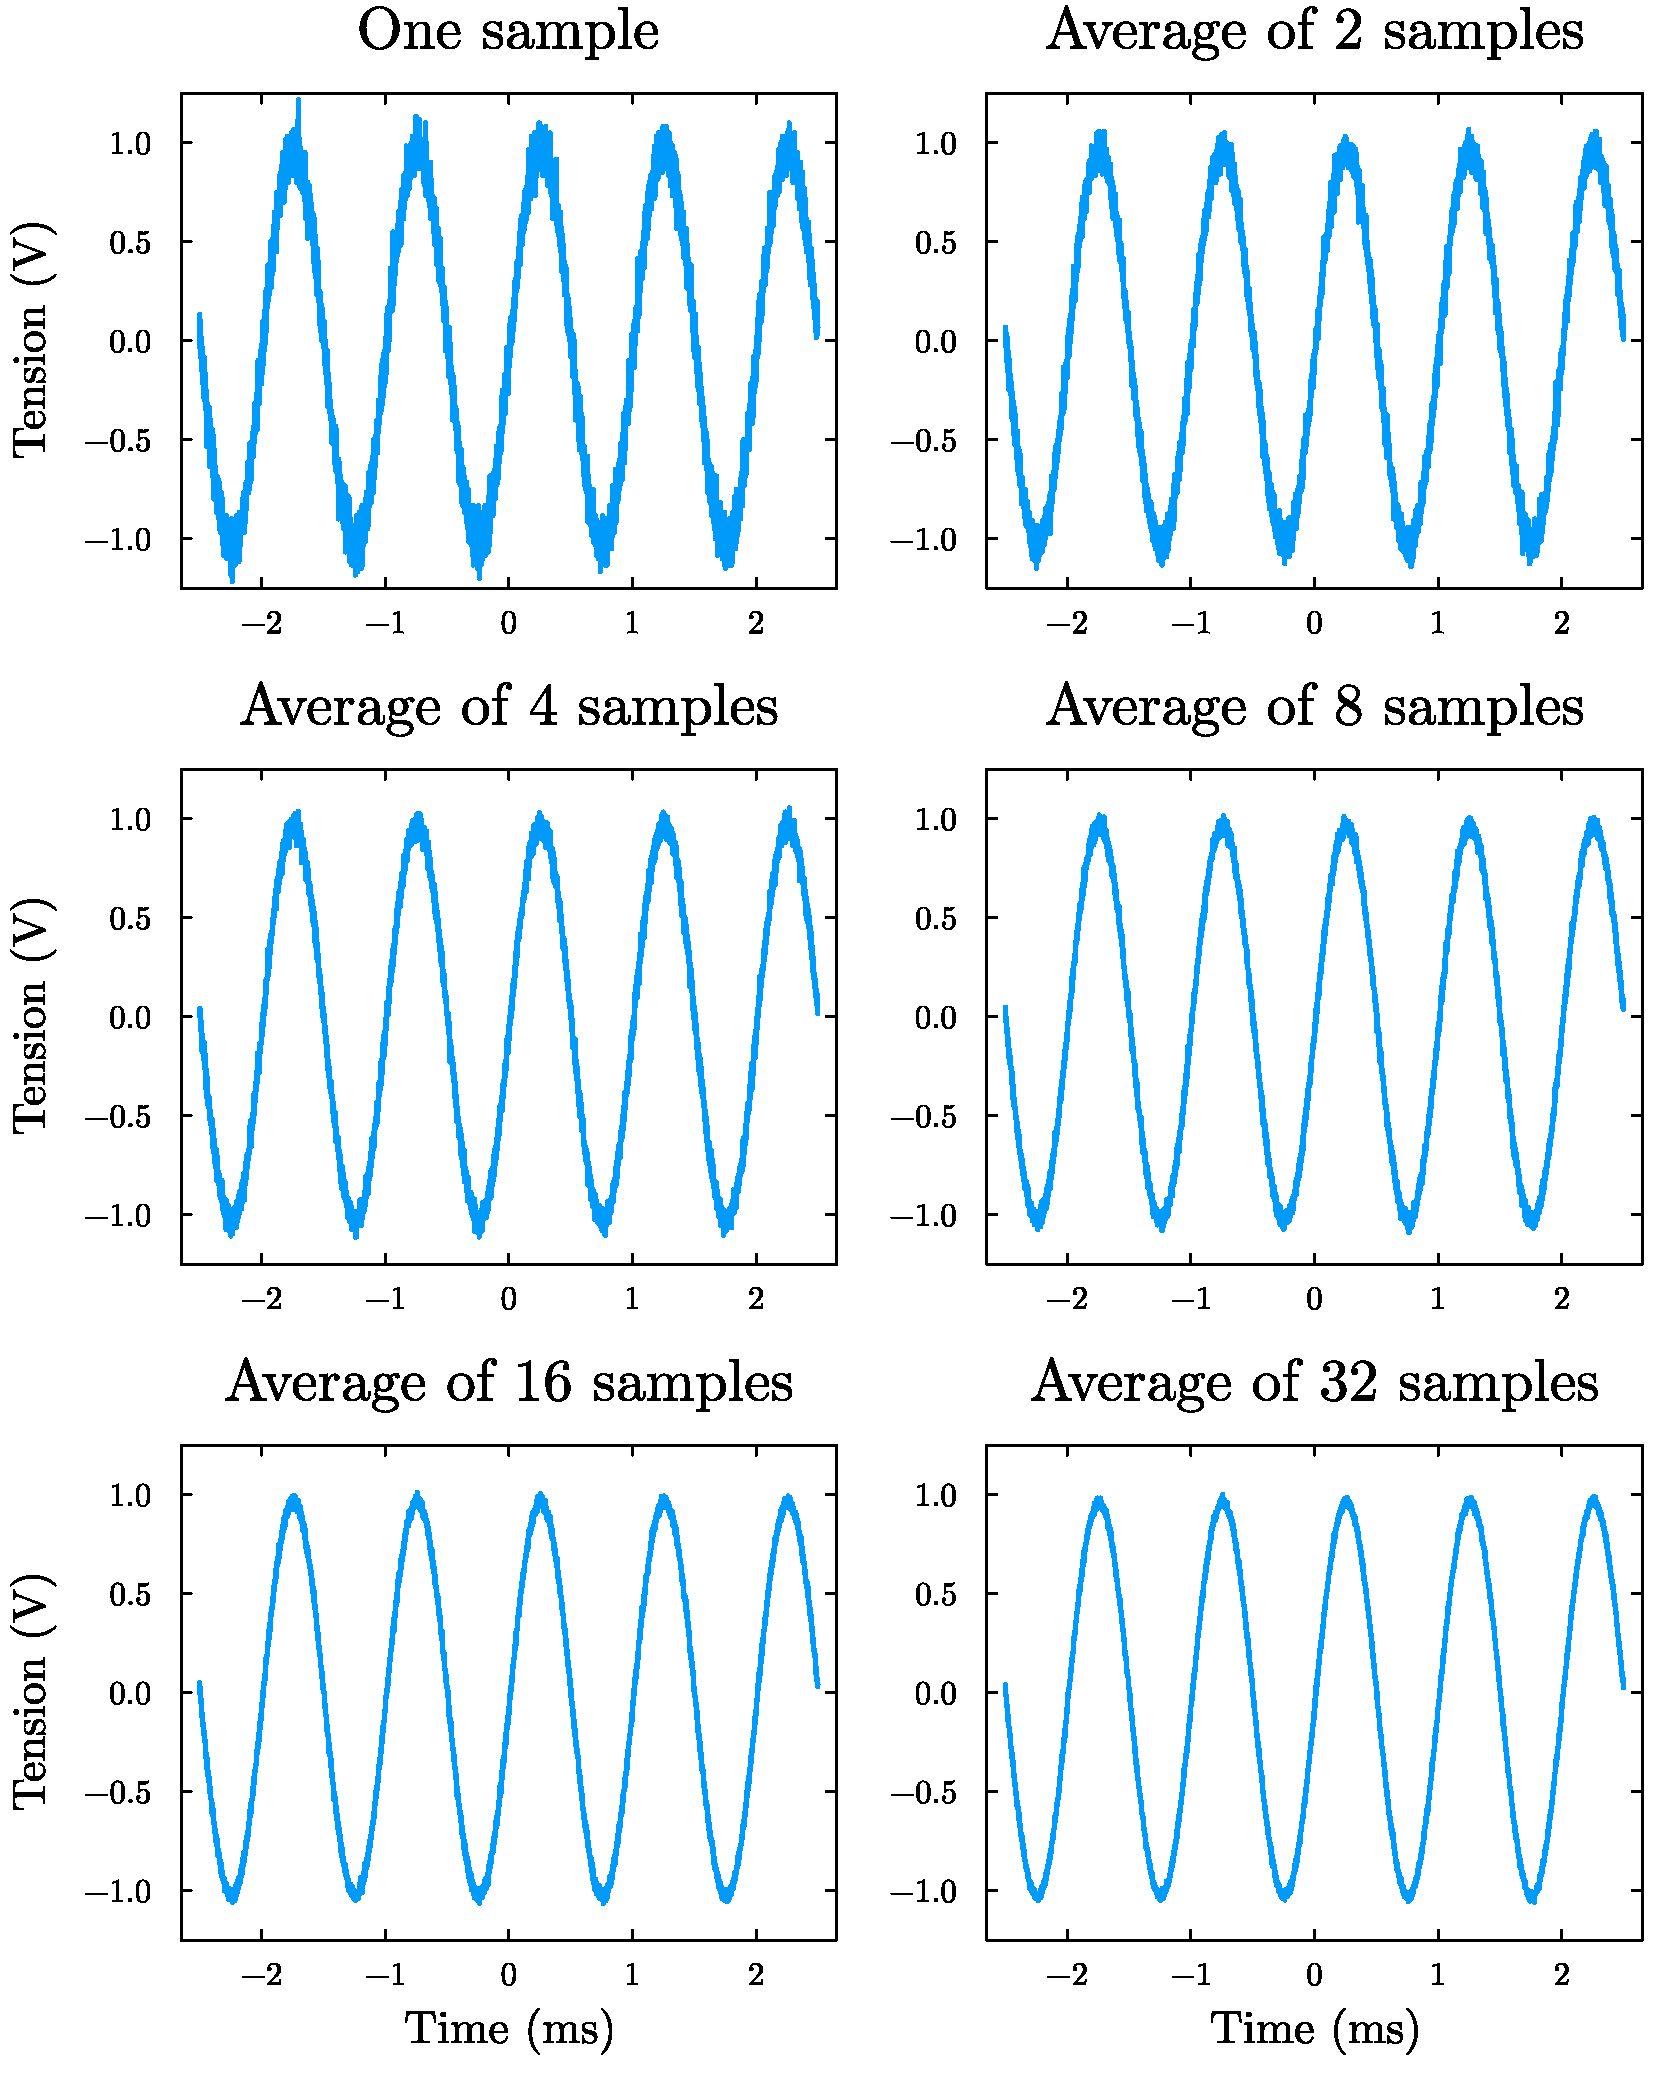
\includegraphics[width=1\textwidth]{Signal_fix.pdf}
    \caption{Signal obtained from the average of different numbers of signal datasets.}
    \label{plot:Noise_decay_signal}
\end{figure}


\end{document}